\documentclass{beamer}
\usepackage{color,amsmath}
\usepackage{subfigure}
\usepackage{booktabs}
\usepackage{framed}
\usepackage{comment}

\def\vf{\vfill}

\newcommand{\goals}{
\begin{itemize}
\item SWBAT \emph{explain} why ethics is important in CSS
\item SWBAT \emph{apply} ethical principles and frameworks to specific research projects
\item SWBAT \emph{describe} approaches to common ethical challenges
\end{itemize}
}

%%%%%%%%%%%%%%%%%%%%%%%%%%
\title[]{Soc 596: Computational Social Science}
\author[]{Matthew J. Salganik\\Department of Sociology\\Princeton University}
\date[]{01-03-Ethics
\vfill
\begin{flushright}
\vspace{0.6in}

\includegraphics[width=0.1\textwidth]{figures/cc.png}
\end{flushright}
}
\begin{document}
%%%%%%%%%%%%%%%%%%%%%%%%%%
\frame{\titlepage}
%%%%%%%%%%%%%%%%%%%%%%%%%%
\begin{frame}

\goals

\end{frame}
%%%%%%%%%%%%%%%%%%%%%%%%%%
\begin{frame}

\begin{center}
Think about ethics as continuous not discrete
\end{center}

\end{frame}
%%%%%%%%%%%%%%%%%%%%%%%%%%
\begin{frame}

\begin{center}
\LARGE{Why care about ethics?}
\end{center}

\end{frame}
%%%%%%%%%%%%%%%%%%%%%%%%%%
\begin{frame}

In the past, what we could do has been the limitation, increasingly what we should do will be the limitation.\\
Research ethics will become increasingly central; it will become harder and harder to avoid.\\
 
\end{frame}
%%%%%%%%%%%%%%%%%%%%%%%%%%
\begin{frame}

I want you to be able to:
\begin{itemize}
\item design ethically thoughtful research 
\item explain your decisions to others
\end{itemize}
 
\end{frame}
%%%%%%%%%%%%%%%%%%%%%%%%%%
\begin{frame}

\begin{itemize}
\item Rules-based approach
\item Ad-hoc approach
\item Principles-based approach
\end{itemize}

\end{frame}
%%%%%%%%%%%%%%%%%%%%%%%%%%
\begin{frame}

\begin{itemize}
\item Emotional contagion
\item Taste, Ties, and Time
\item Encore
\pause
\item Think-pair-share other examples?
\end{itemize}

\end{frame}
%%%%%%%%%%%%%%%%%%%%%%%%%%%
\begin{frame}

Consider Emotional contagion.
\begin{center}
\LARGE{Should academic researchers and companies follow the same rules?}
\end{center}

Think-pair-share

\end{frame}
%%%%%%%%%%%%%%%%%%%%%%%%%%%
\begin{frame}

\begin{center}
\LARGE{How should we handle these challenges?}
\end{center}

\end{frame}
%%%%%%%%%%%%%%%%%%%%%%%%%%%
\begin{frame}

\begin{center}
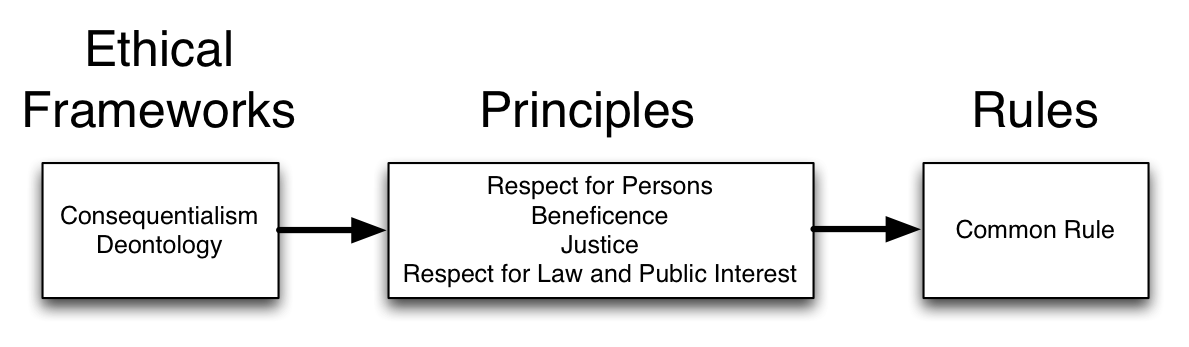
\includegraphics[width=0.9\textwidth]{figures/ethics_schematic_simple.png}
\end{center}

\end{frame}
%%%%%%%%%%%%%%%%%%%%%%%%%%%
\begin{frame}

\begin{itemize}
\item Respect for persons
\end{itemize}

\end{frame}
%%%%%%%%%%%%%%%%%%%%%%%%%%
\begin{frame}

Respect for persons:\\
Participants decide not you

\end{frame}
%%%%%%%%%%%%%%%%%%%%%%%%%%
\begin{frame}

\begin{itemize}
\item Respect for persons
\item Beneficence
\end{itemize}

\end{frame}
%%%%%%%%%%%%%%%%%%%%%%%%%%
\begin{frame}

Beneficence:\\
Minimize risk, maximize benefits, then decide

\end{frame}
%%%%%%%%%%%%%%%%%%%%%%%%%%
\begin{frame}

\begin{itemize}
\item Respect for persons
\item Beneficence
\item Justice
\end{itemize}

\end{frame}
%%%%%%%%%%%%%%%%%%%%%%%%%%
\begin{frame}

Justice:\\
distribution of burdens and benefits of research
\pause
\begin{itemize}
\item poorly educated and disenfranchised citizens
\item prisoners
\item institutionalized and mentally disabled children
\item old and debilitated hospital patients
\end{itemize}
\pause
Also includes access to benefits of research

\end{frame}
%%%%%%%%%%%%%%%%%%%%%%%%%%
\begin{frame}

\begin{itemize}
\item Respect for persons
\item Beneficence
\item Justice
\item Respect for Law and Public Interest
\end{itemize}

\end{frame}
%%%%%%%%%%%%%%%%%%%%%%%%%
\begin{frame}

Terms of service agreements

\end{frame}
%%%%%%%%%%%%%%%%%%%%%%%%%
\begin{frame}

\begin{center}
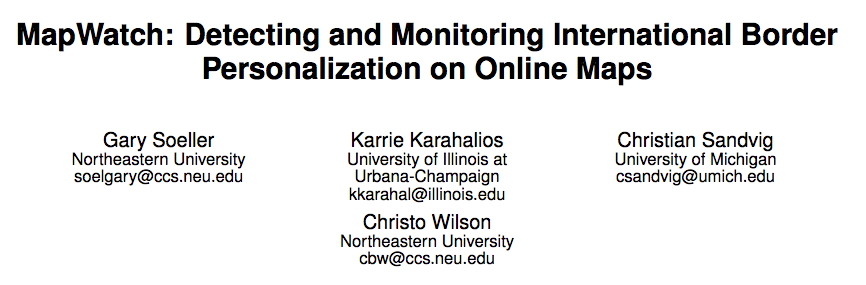
\includegraphics[width=0.9\textwidth]{figures/soeller_mapwatch_2016_title.png}
\end{center}

\vf
\url{http://dx.doi.org/10.1145/2872427.2883016}
\end{frame}
%%%%%%%%%%%%%%%%%%%%%%%%%
\begin{frame}

Abstract:\\
``Maps have long played a crucial role in enabling people to conceptualize and navigate the world around them. However, maps also encode the world-views of their creators. Disputed international borders are one example of this: governments may mandate that cartographers produce maps that conform to their view of a territorial dispute. Today, online maps maintained by private corporations have become the norm. However, these new maps are still subject to old debates. Companies like Google and Bing resolve these disputes by localizing their maps to meet government requirements and user preferences, i.e., users in different locations are shown maps with different international boundaries. We argue that this non-transparent personalization of maps may exacerbate nationalistic disputes by promoting divergent views of geopolitical realities.''

\end{frame}
%%%%%%%%%%%%%%%%%%%%%%%
\begin{frame}

Abstract, part 2:\\
``To address this problem, we present MapWatch, our system for detecting and cataloging personalization of international borders in online maps. Our system continuously crawls all map tiles from Google and Bing maps, and leverages crowdworkers to identify border personalization. In this paper, we present the architecture of MapWatch, and analyze the instances of border personalization on Google and Bing, including one border change that MapWatch identified live, as Google was rolling out the update.''

\end{frame}
%%%%%%%%%%%%%%%%%%%%%%%%%
\begin{frame}

\begin{center}
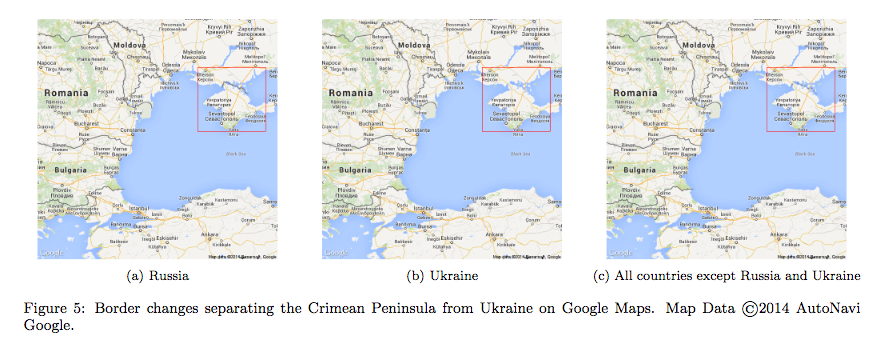
\includegraphics[width=0.9\textwidth]{figures/soeller_mapwatch_2016_fig5.png}
\end{center}

\vf
\url{http://dx.doi.org/10.1145/2872427.2883016}
\end{frame}
%%%%%%%%%%%%%%%%%%%%%%%%%
\begin{frame}

\begin{center}
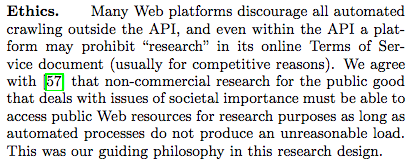
\includegraphics[width=0.9\textwidth]{figures/soeller_mapwatch_2016_ethics.png}
\end{center}

\vf
\url{http://dx.doi.org/10.1145/2872427.2883016}
\end{frame}
%%%%%%%%%%%%%%%%%%%%%%%%%
\begin{frame}

Researchers (with the support of the ACLU) have filed a case challenging the CFAA, Sandivg v Lynch:\\
\tiny{\textcolor{blue}{\url{https://www.aclu.org/cases/sandvig-v-lynch-challenge-cfaa-prohibition-uncovering-racial-discrimination-online}}}

\end{frame}
%%%%%%%%%%%%%%%%%%%%%%%%%%
\begin{frame}

\begin{itemize}
\item Respect for persons
\item Beneficence
\item Justice
\item Respect for Law and Public Interest
\end{itemize}

\vf
How do you balance these four principles?

\end{frame}
%%%%%%%%%%%%%%%%%%%%%%%%%
\begin{frame}

\begin{itemize}
\item Consequentialism
\item Deontology
\end{itemize}

\end{frame}
%%%%%%%%%%%%%%%%%%%%%%%%%
\begin{frame}

\begin{center}
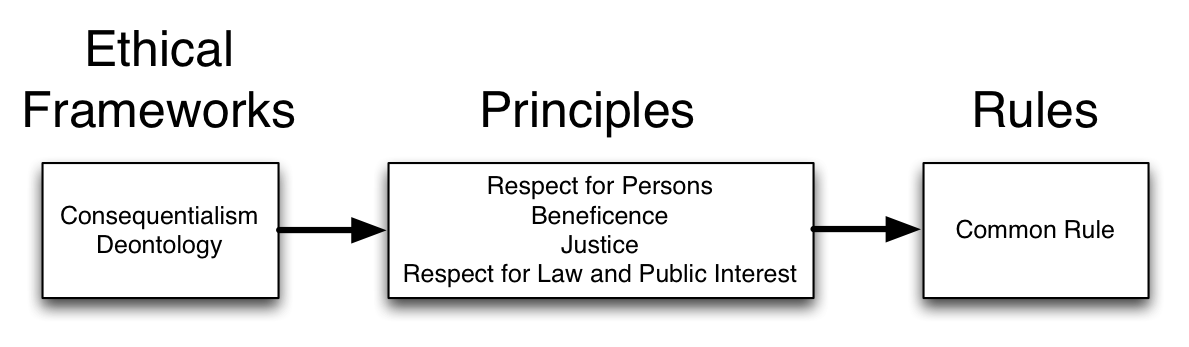
\includegraphics[width=0.9\textwidth]{figures/ethics_schematic_simple.png}
\end{center}

\end{frame}
%%%%%%%%%%%%%%%%%%%%%%%%%
\begin{frame}

Informed consent

\end{frame}
%%%%%%%%%%%%%%%%%%%%%%%%%%%
\begin{frame}

Understanding and managing informational risk

\end{frame}
%%%%%%%%%%%%%%%%%%%%%%%%%%%
\begin{frame}

\begin{center}
\only<1>{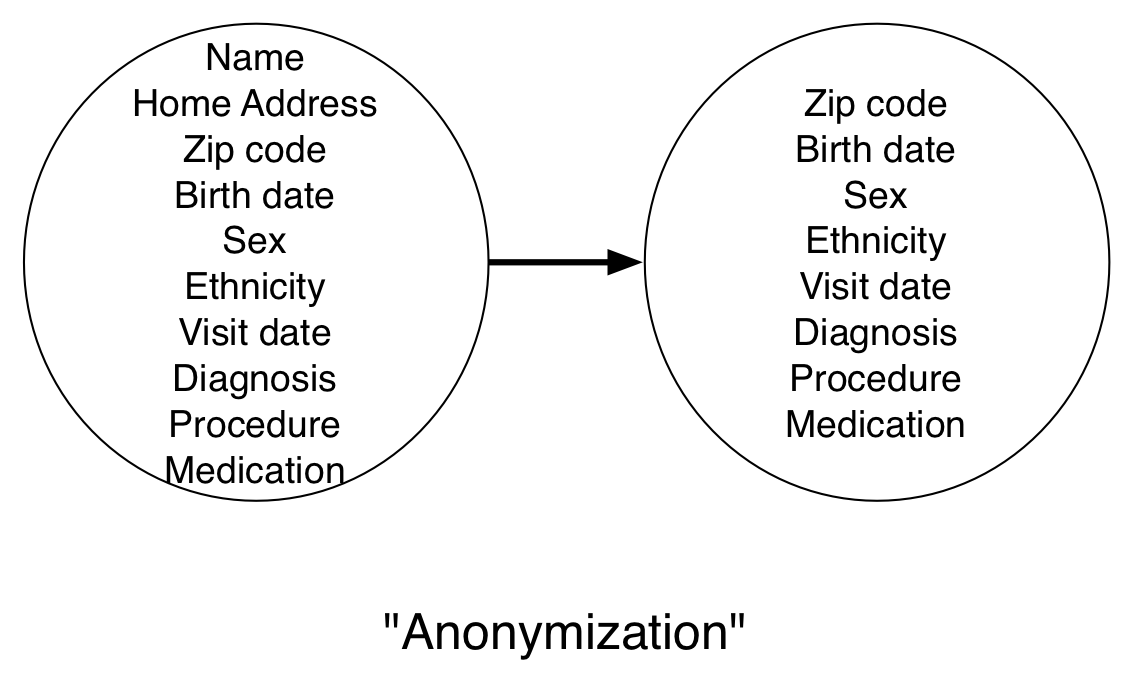
\includegraphics[width=0.9\textwidth]{figures/anonymization.png}}
\only<2>{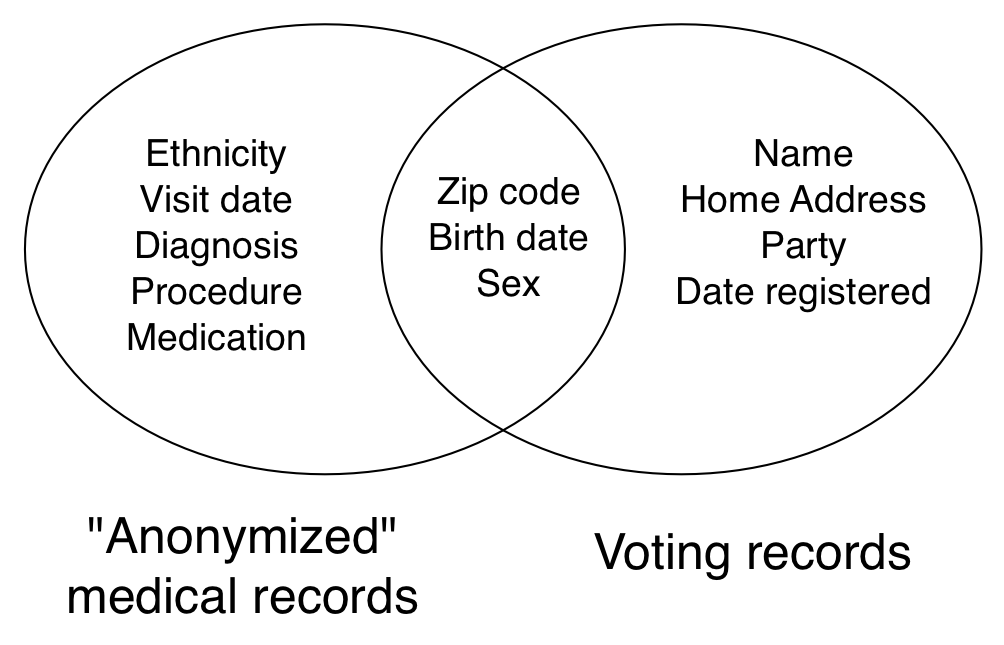
\includegraphics[width=0.9\textwidth]{figures/re-identified.png}}
\end{center}

\end{frame}
%%%%%%%%%%%%%%%%%%%%%%%%%%%
\begin{frame}

Privacy

\end{frame}
%%%%%%%%%%%%%%%%%%%%%%%%%%%
\begin{frame}

Making decisions in the face of uncertainty

\end{frame}
%%%%%%%%%%%%%%%%%%%%%%%%%%%
\begin{frame}

\begin{itemize}
\item IRB is a floor not a ceiling
\pause
\item Put yourself in everyone else's shoes
\pause
\item Think of research ethics as continuous not discrete
\end{itemize}

\end{frame}
%%%%%%%%%%%%%%%%%%%%%%%%%%%
\begin{frame}

\goals

\end{frame}
%%%%%%%%%%%%%%%%%%%%%%%%%%%


%%%%%%%%%%%%%%%%%%%%%%%%%%
%%%%%%%%%%%%%%%%%%%%%%%%%%
%%%%%%%%%%%%%%%%%%%%%%%%%%
%%%%%%%%%%%%%%%%%%%%%%%%%%
%%%%%%%%%%%%%%%%%%%%%%%%%%
%%%%%%%%%%%%%%%%%%%%%%%%%%


\end{document}
